\documentclass[12pt,]{article}
\usepackage{lmodern}
\usepackage{amssymb,amsmath}
\usepackage{ifxetex,ifluatex}
\usepackage{fixltx2e} % provides \textsubscript
\ifnum 0\ifxetex 1\fi\ifluatex 1\fi=0 % if pdftex
  \usepackage[T1]{fontenc}
  \usepackage[utf8]{inputenc}
\else % if luatex or xelatex
  \ifxetex
    \usepackage{mathspec}
  \else
    \usepackage{fontspec}
  \fi
  \defaultfontfeatures{Ligatures=TeX,Scale=MatchLowercase}
\fi
% use upquote if available, for straight quotes in verbatim environments
\IfFileExists{upquote.sty}{\usepackage{upquote}}{}
% use microtype if available
\IfFileExists{microtype.sty}{%
\usepackage{microtype}
\UseMicrotypeSet[protrusion]{basicmath} % disable protrusion for tt fonts
}{}
\usepackage[margin=1.0in]{geometry}
\usepackage{hyperref}
\hypersetup{unicode=true,
            pdftitle={Supplementary Information},
            pdfborder={0 0 0},
            breaklinks=true}
\urlstyle{same}  % don't use monospace font for urls
\usepackage{graphicx,grffile}
\makeatletter
\def\maxwidth{\ifdim\Gin@nat@width>\linewidth\linewidth\else\Gin@nat@width\fi}
\def\maxheight{\ifdim\Gin@nat@height>\textheight\textheight\else\Gin@nat@height\fi}
\makeatother
% Scale images if necessary, so that they will not overflow the page
% margins by default, and it is still possible to overwrite the defaults
% using explicit options in \includegraphics[width, height, ...]{}
\setkeys{Gin}{width=\maxwidth,height=\maxheight,keepaspectratio}
\IfFileExists{parskip.sty}{%
\usepackage{parskip}
}{% else
\setlength{\parindent}{0pt}
\setlength{\parskip}{6pt plus 2pt minus 1pt}
}
\setlength{\emergencystretch}{3em}  % prevent overfull lines
\providecommand{\tightlist}{%
  \setlength{\itemsep}{0pt}\setlength{\parskip}{0pt}}
\setcounter{secnumdepth}{0}
% Redefines (sub)paragraphs to behave more like sections
\ifx\paragraph\undefined\else
\let\oldparagraph\paragraph
\renewcommand{\paragraph}[1]{\oldparagraph{#1}\mbox{}}
\fi
\ifx\subparagraph\undefined\else
\let\oldsubparagraph\subparagraph
\renewcommand{\subparagraph}[1]{\oldsubparagraph{#1}\mbox{}}
\fi

%%% Use protect on footnotes to avoid problems with footnotes in titles
\let\rmarkdownfootnote\footnote%
\def\footnote{\protect\rmarkdownfootnote}

%%% Change title format to be more compact
\usepackage{titling}

% Create subtitle command for use in maketitle
\providecommand{\subtitle}[1]{
  \posttitle{
    \begin{center}\large#1\end{center}
    }
}

\setlength{\droptitle}{-2em}

  \title{\textbf{Supplementary Information}}
    \pretitle{\vspace{\droptitle}\centering\huge}
  \posttitle{\par}
  \subtitle{\textbf{Seasonal Dynamics of Epiphytic Microbial Communities on Marine
Macrophyte Surfaces}}
  \author{}
    \preauthor{}\postauthor{}
    \date{}
    \predate{}\postdate{}
  
\usepackage{times} % Times New Roman font
\usepackage[T1]{fontenc}

\usepackage[none]{hyphenat}

\usepackage{setspace}
\doublespacing
\setlength{\parskip}{1em}

\usepackage{lineno}

\usepackage{pdfpages}

\usepackage{indentfirst}

\usepackage[labelsep=period, labelfont=bf]{caption}
\renewcommand{\thefigure}{S\arabic{figure}}
\renewcommand{\thetable}{S\arabic{table}}
\captionsetup{justification=raggedright,singlelinecheck=false}

\usepackage{pdflscape}
\newcommand{\blandscape}{\begin{landscape}}
\newcommand{\elandscape}{\end{landscape}}

\usepackage{siunitx}
\DeclareSIUnit\molar{\mole\per\cubic\deci\metre}
\DeclareSIUnit\Molar{\textsc{m}}
\DeclareSIUnit\cells{\text{cells}}

\usepackage{caption}
\captionsetup{justification=justified}

\usepackage{float}
\usepackage{booktabs}
\usepackage{longtable}
\usepackage{array}
\usepackage{multirow}
\usepackage{wrapfig}
\usepackage{float}
\usepackage{colortbl}
\usepackage{pdflscape}
\usepackage{tabu}
\usepackage{threeparttable}
\usepackage{threeparttablex}
\usepackage[normalem]{ulem}
\usepackage{makecell}
\usepackage{xcolor}

\begin{document}
\maketitle

\vspace{70mm}

\textsuperscript{1\(\dagger\)}

\vspace{40mm}

\(\dagger\) To whom correspondence should be addressed:
\href{mailto:marino.korlevic@irb.hr}{\nolinkurl{marino.korlevic@irb.hr}}

1. Ruđer Bošković Institute, Center for Marine Research, G. Paliaga 5,
Rovinj, Croatia

2. University of Vienna, Department of Limnology and Bio-Oceanography,
Althanstraße 14, Vienna, Austria

\linenumbers
\sisetup{mode=text}
\setlength\parindent{24pt}

\hypertarget{supplementary-figures}{%
\subsection{Supplementary Figures}\label{supplementary-figures}}

\begin{figure}[H]

{\centering 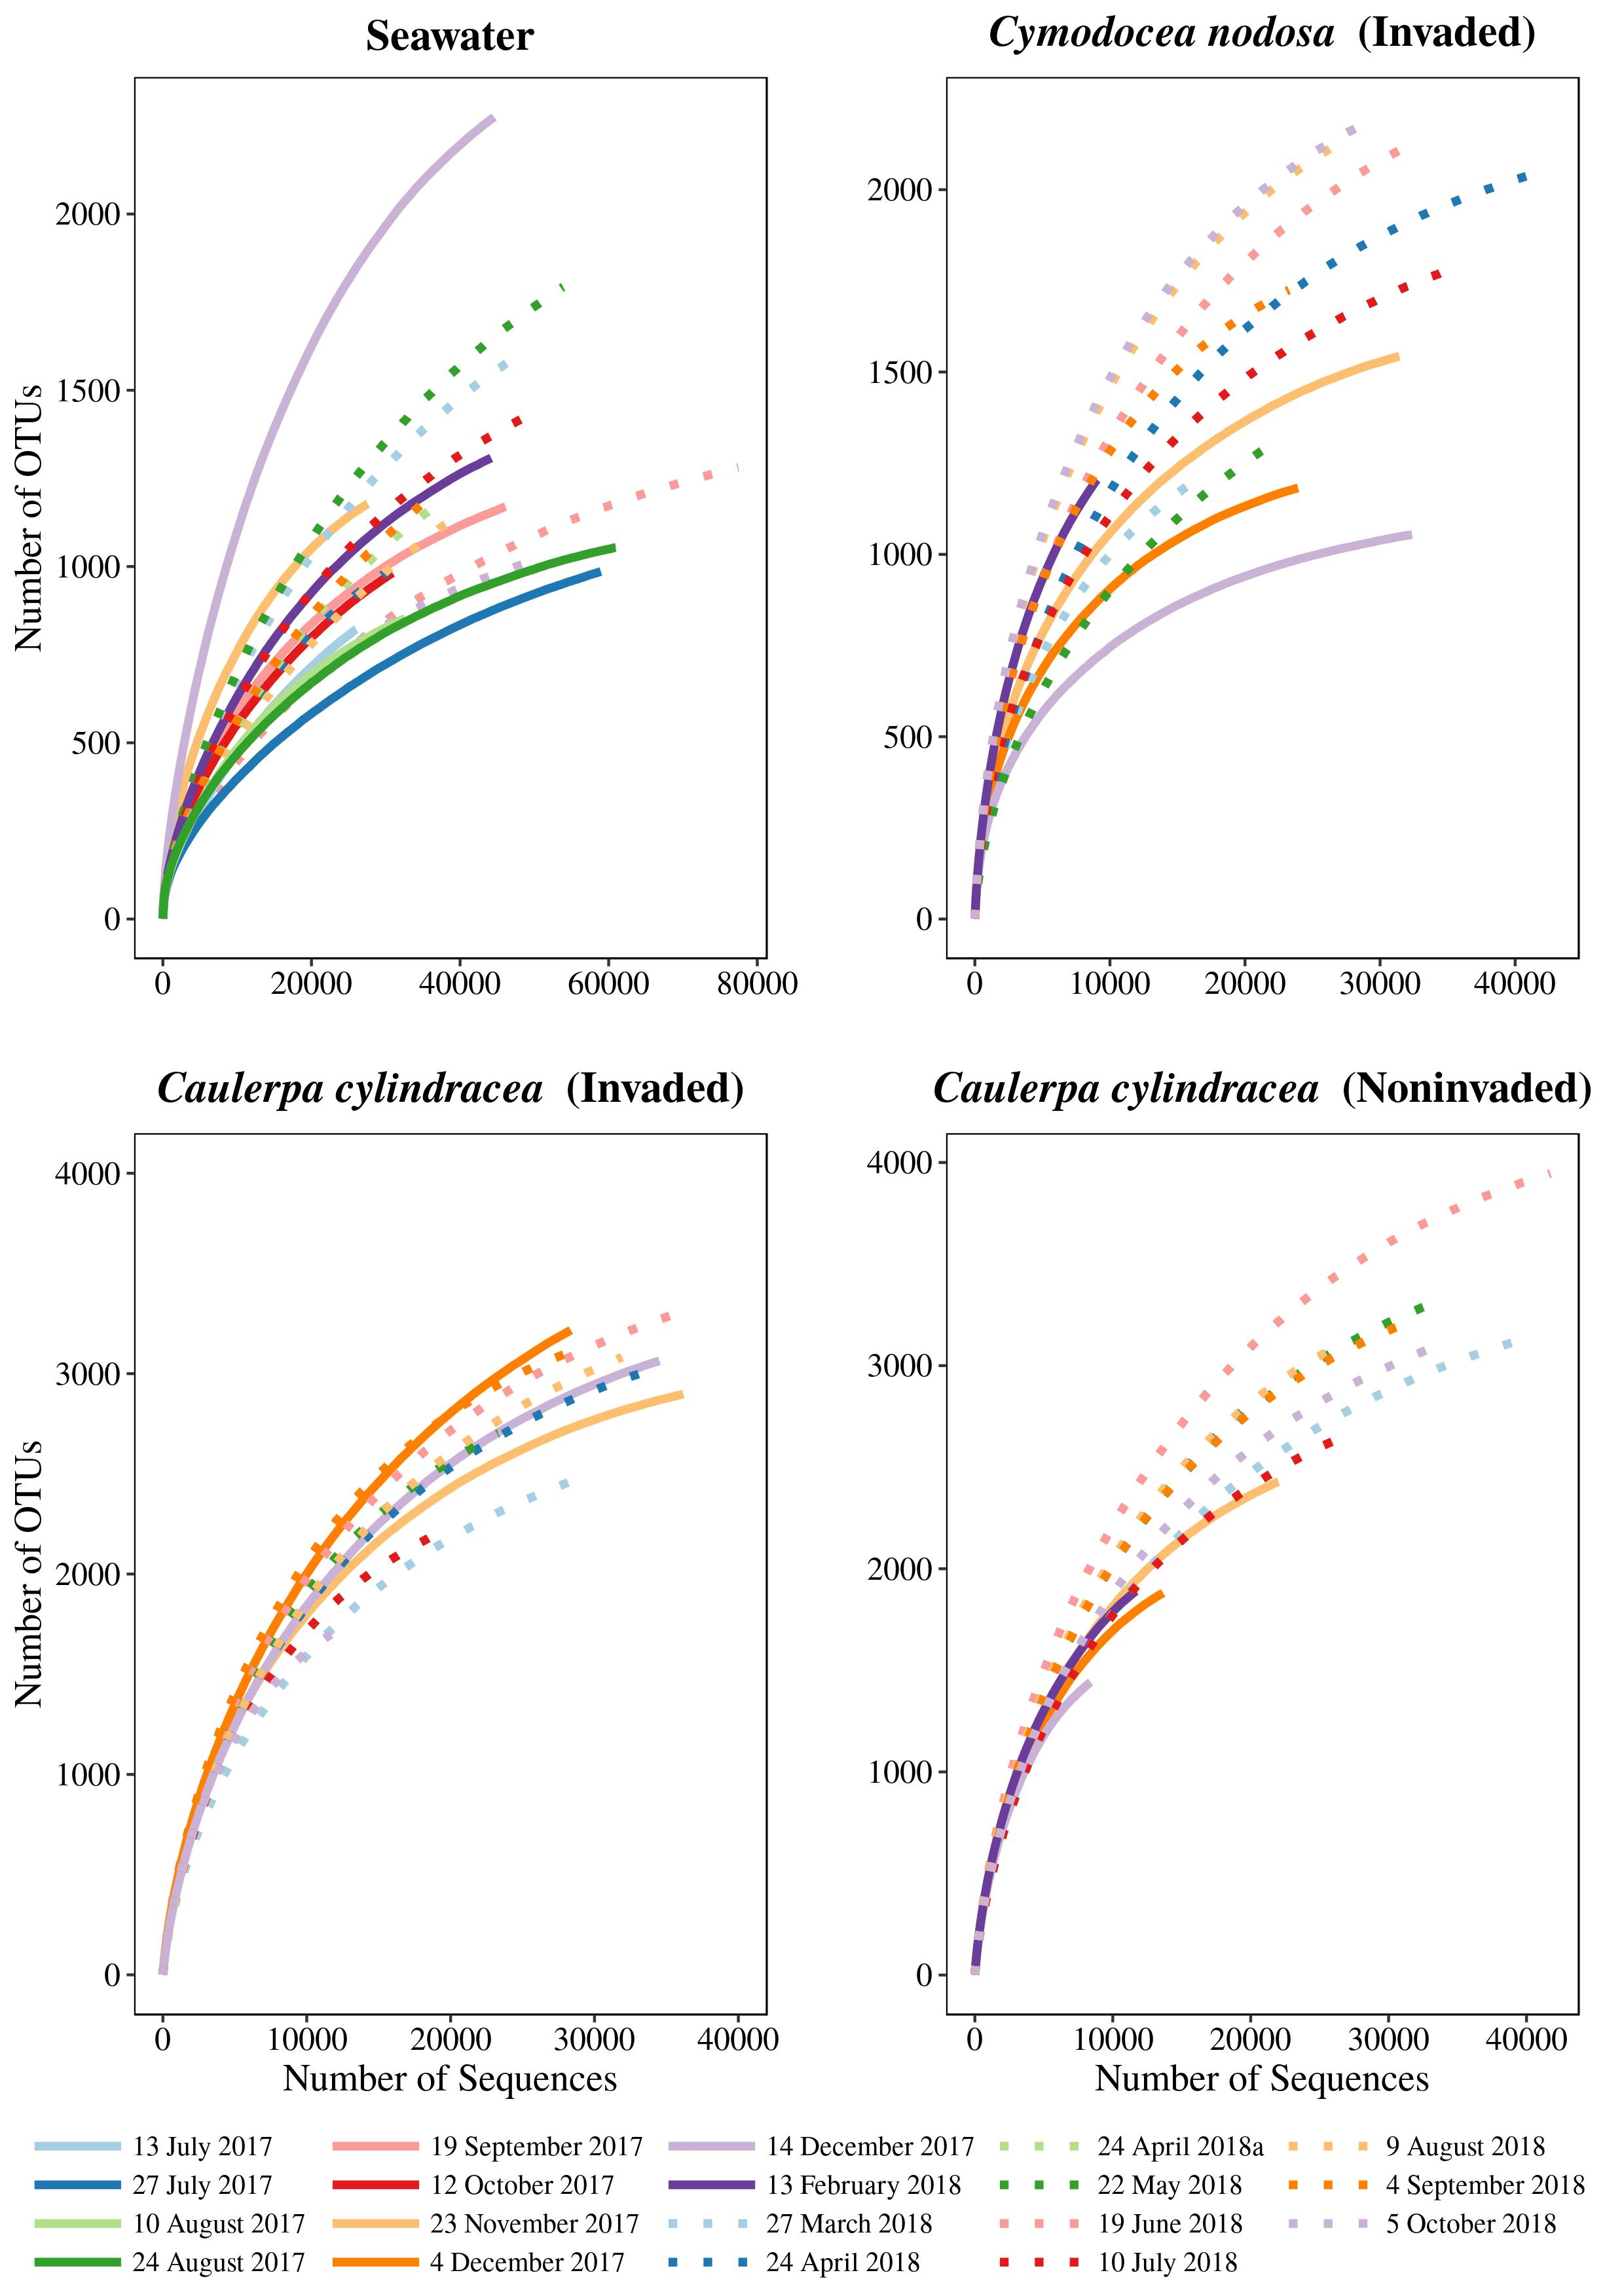
\includegraphics[width=0.85\linewidth]{../results/figures/rarefaction} 

}

\caption{Rarefaction curves of bacterial and archaeal communities from the surfaces of macrophytes (\textit{Cymodocea nodosa} [Invaded] and \textit{Caulerpa cylindracea} [Invaded and Noninvaded]) and in the surrounding seawater.\label{rarefaction}}\label{fig:unnamed-chunk-1}
\end{figure}

\begin{figure}[H]

{\centering 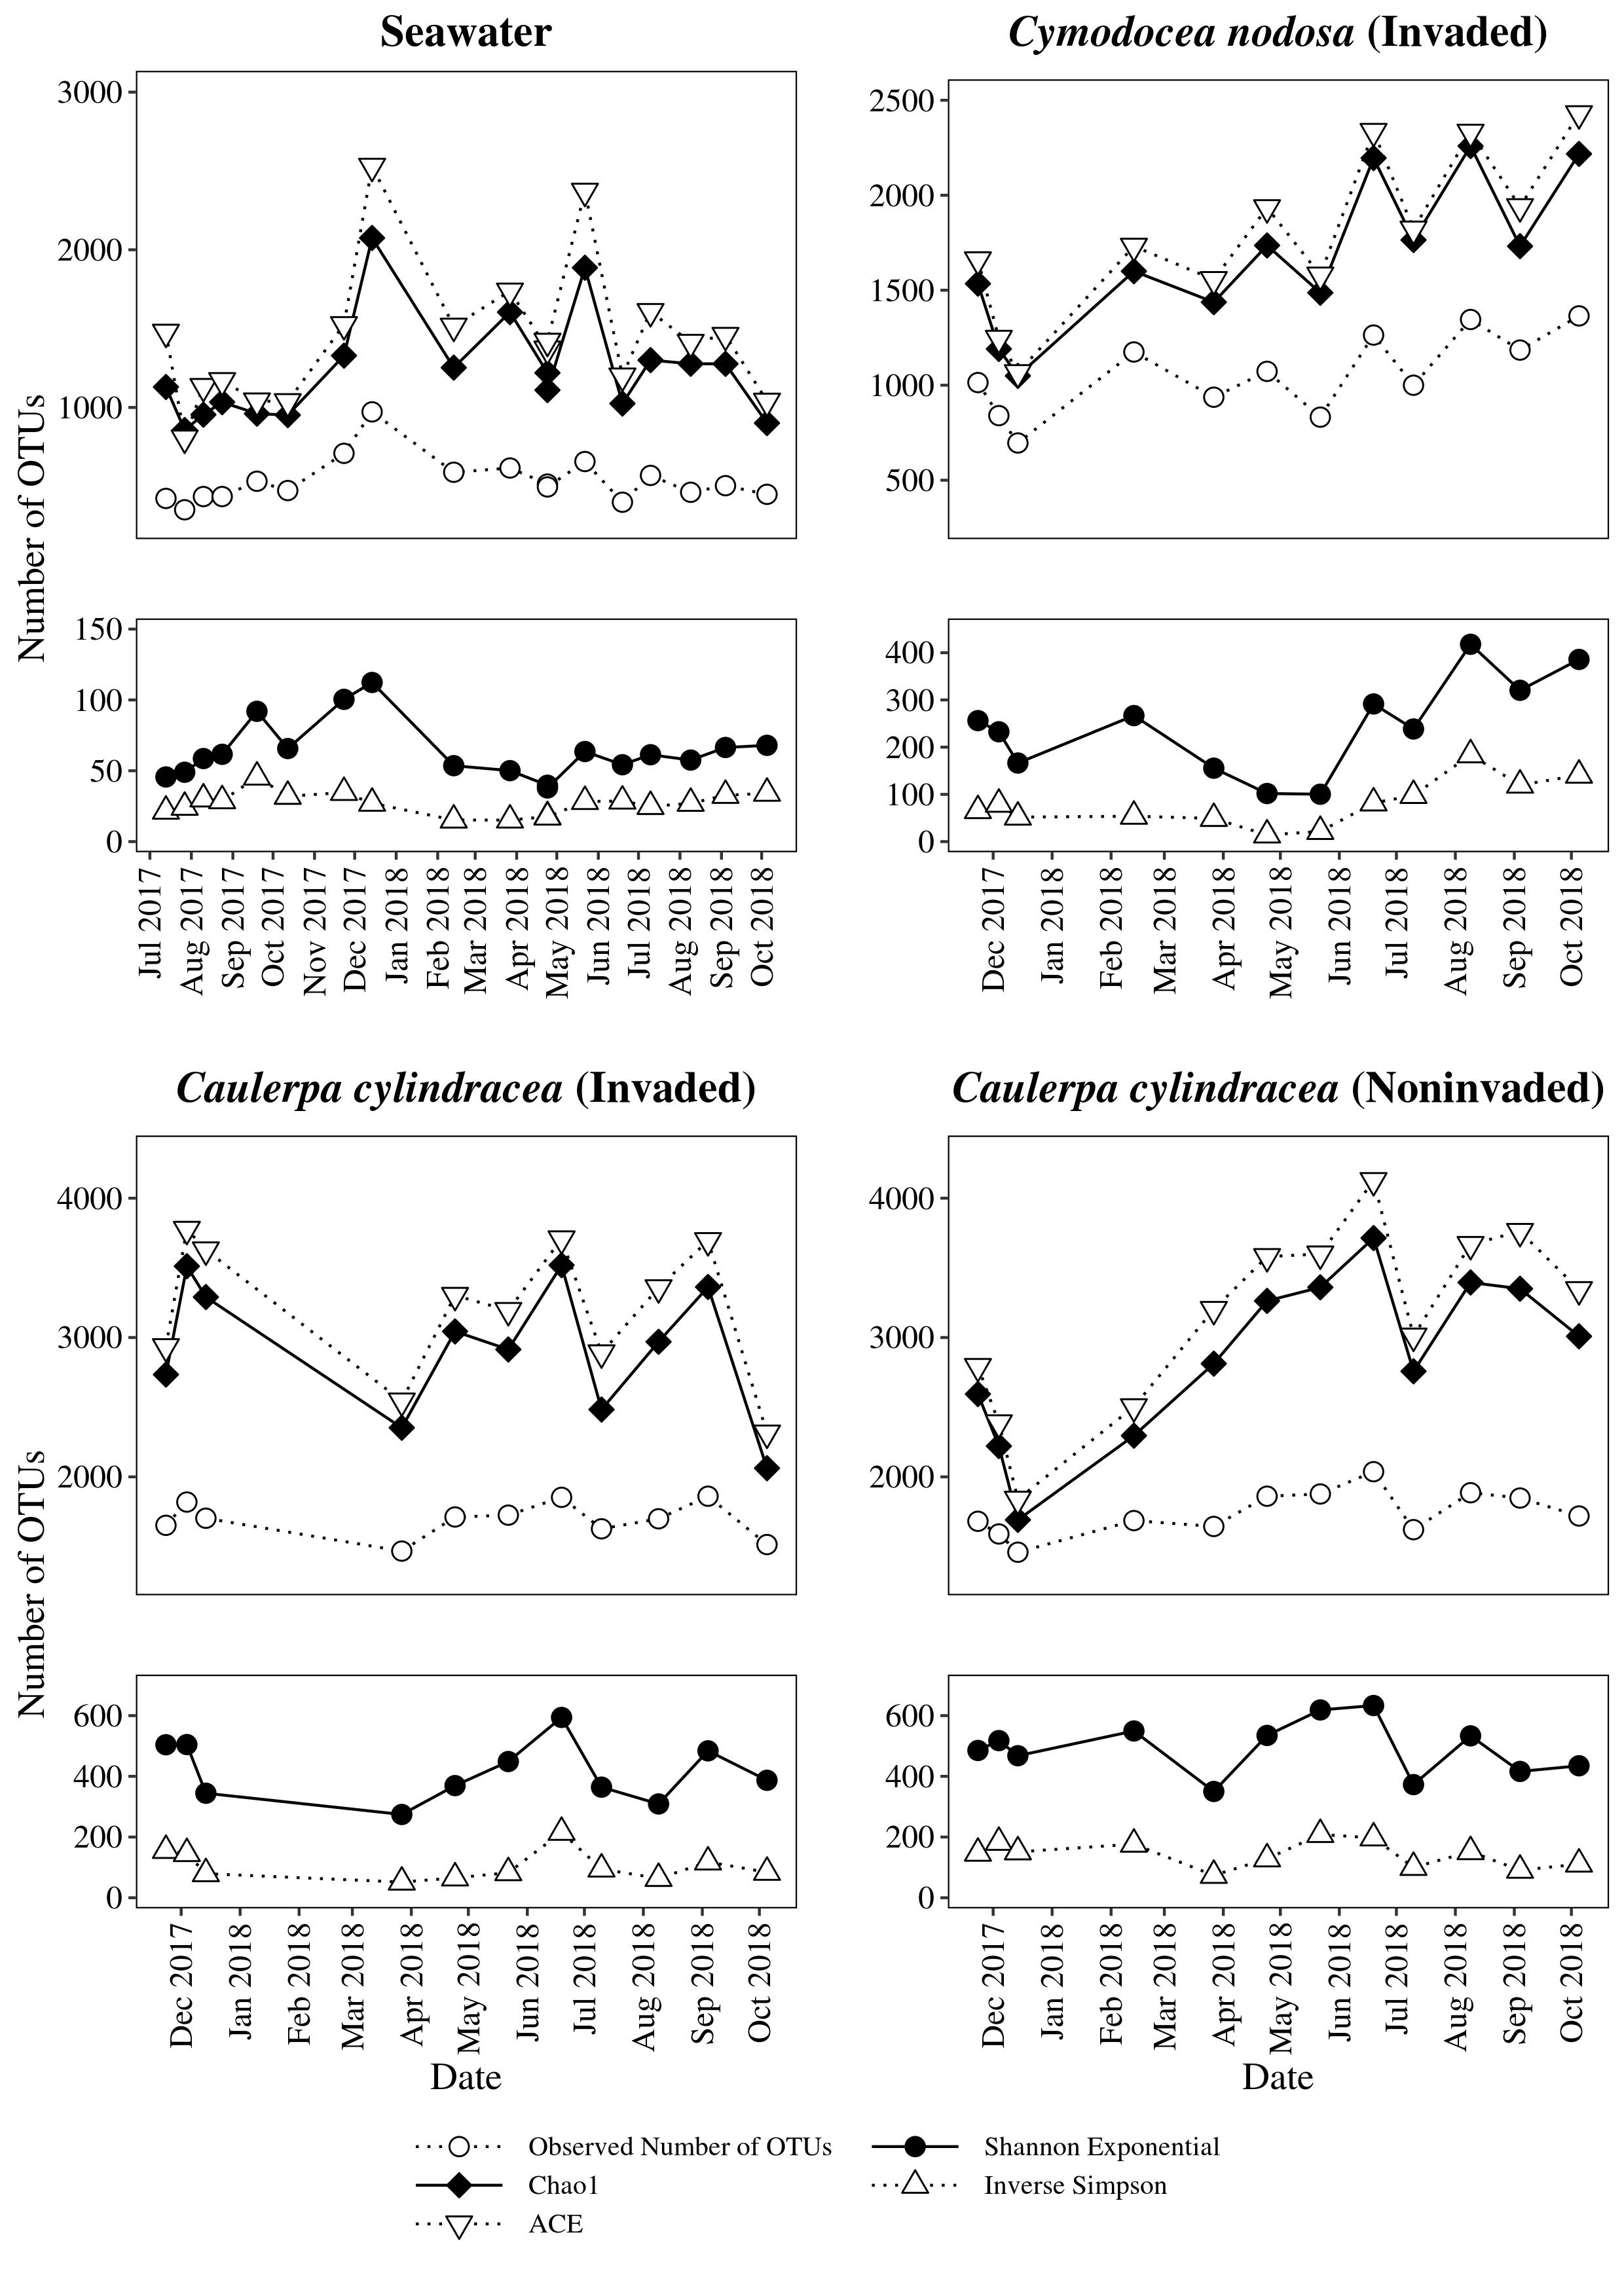
\includegraphics[width=0.85\linewidth]{../results/figures/calculators} 

}

\caption{Seasonal dynamics of observed number of OTUs, Chao1, ACE, exponential of the Shannon Diversity Index and Inverse Simpson Index of bacterial and archaeal communities from the surfaces of macrophytes (\textit{Cymodocea nodosa} [Invaded] and \textit{Caulerpa cylindracea} [Invaded and Noninvaded]) and in the surrounding seawater.\label{calculators}}\label{fig:unnamed-chunk-2}
\end{figure}

\begin{figure}[H]

{\centering 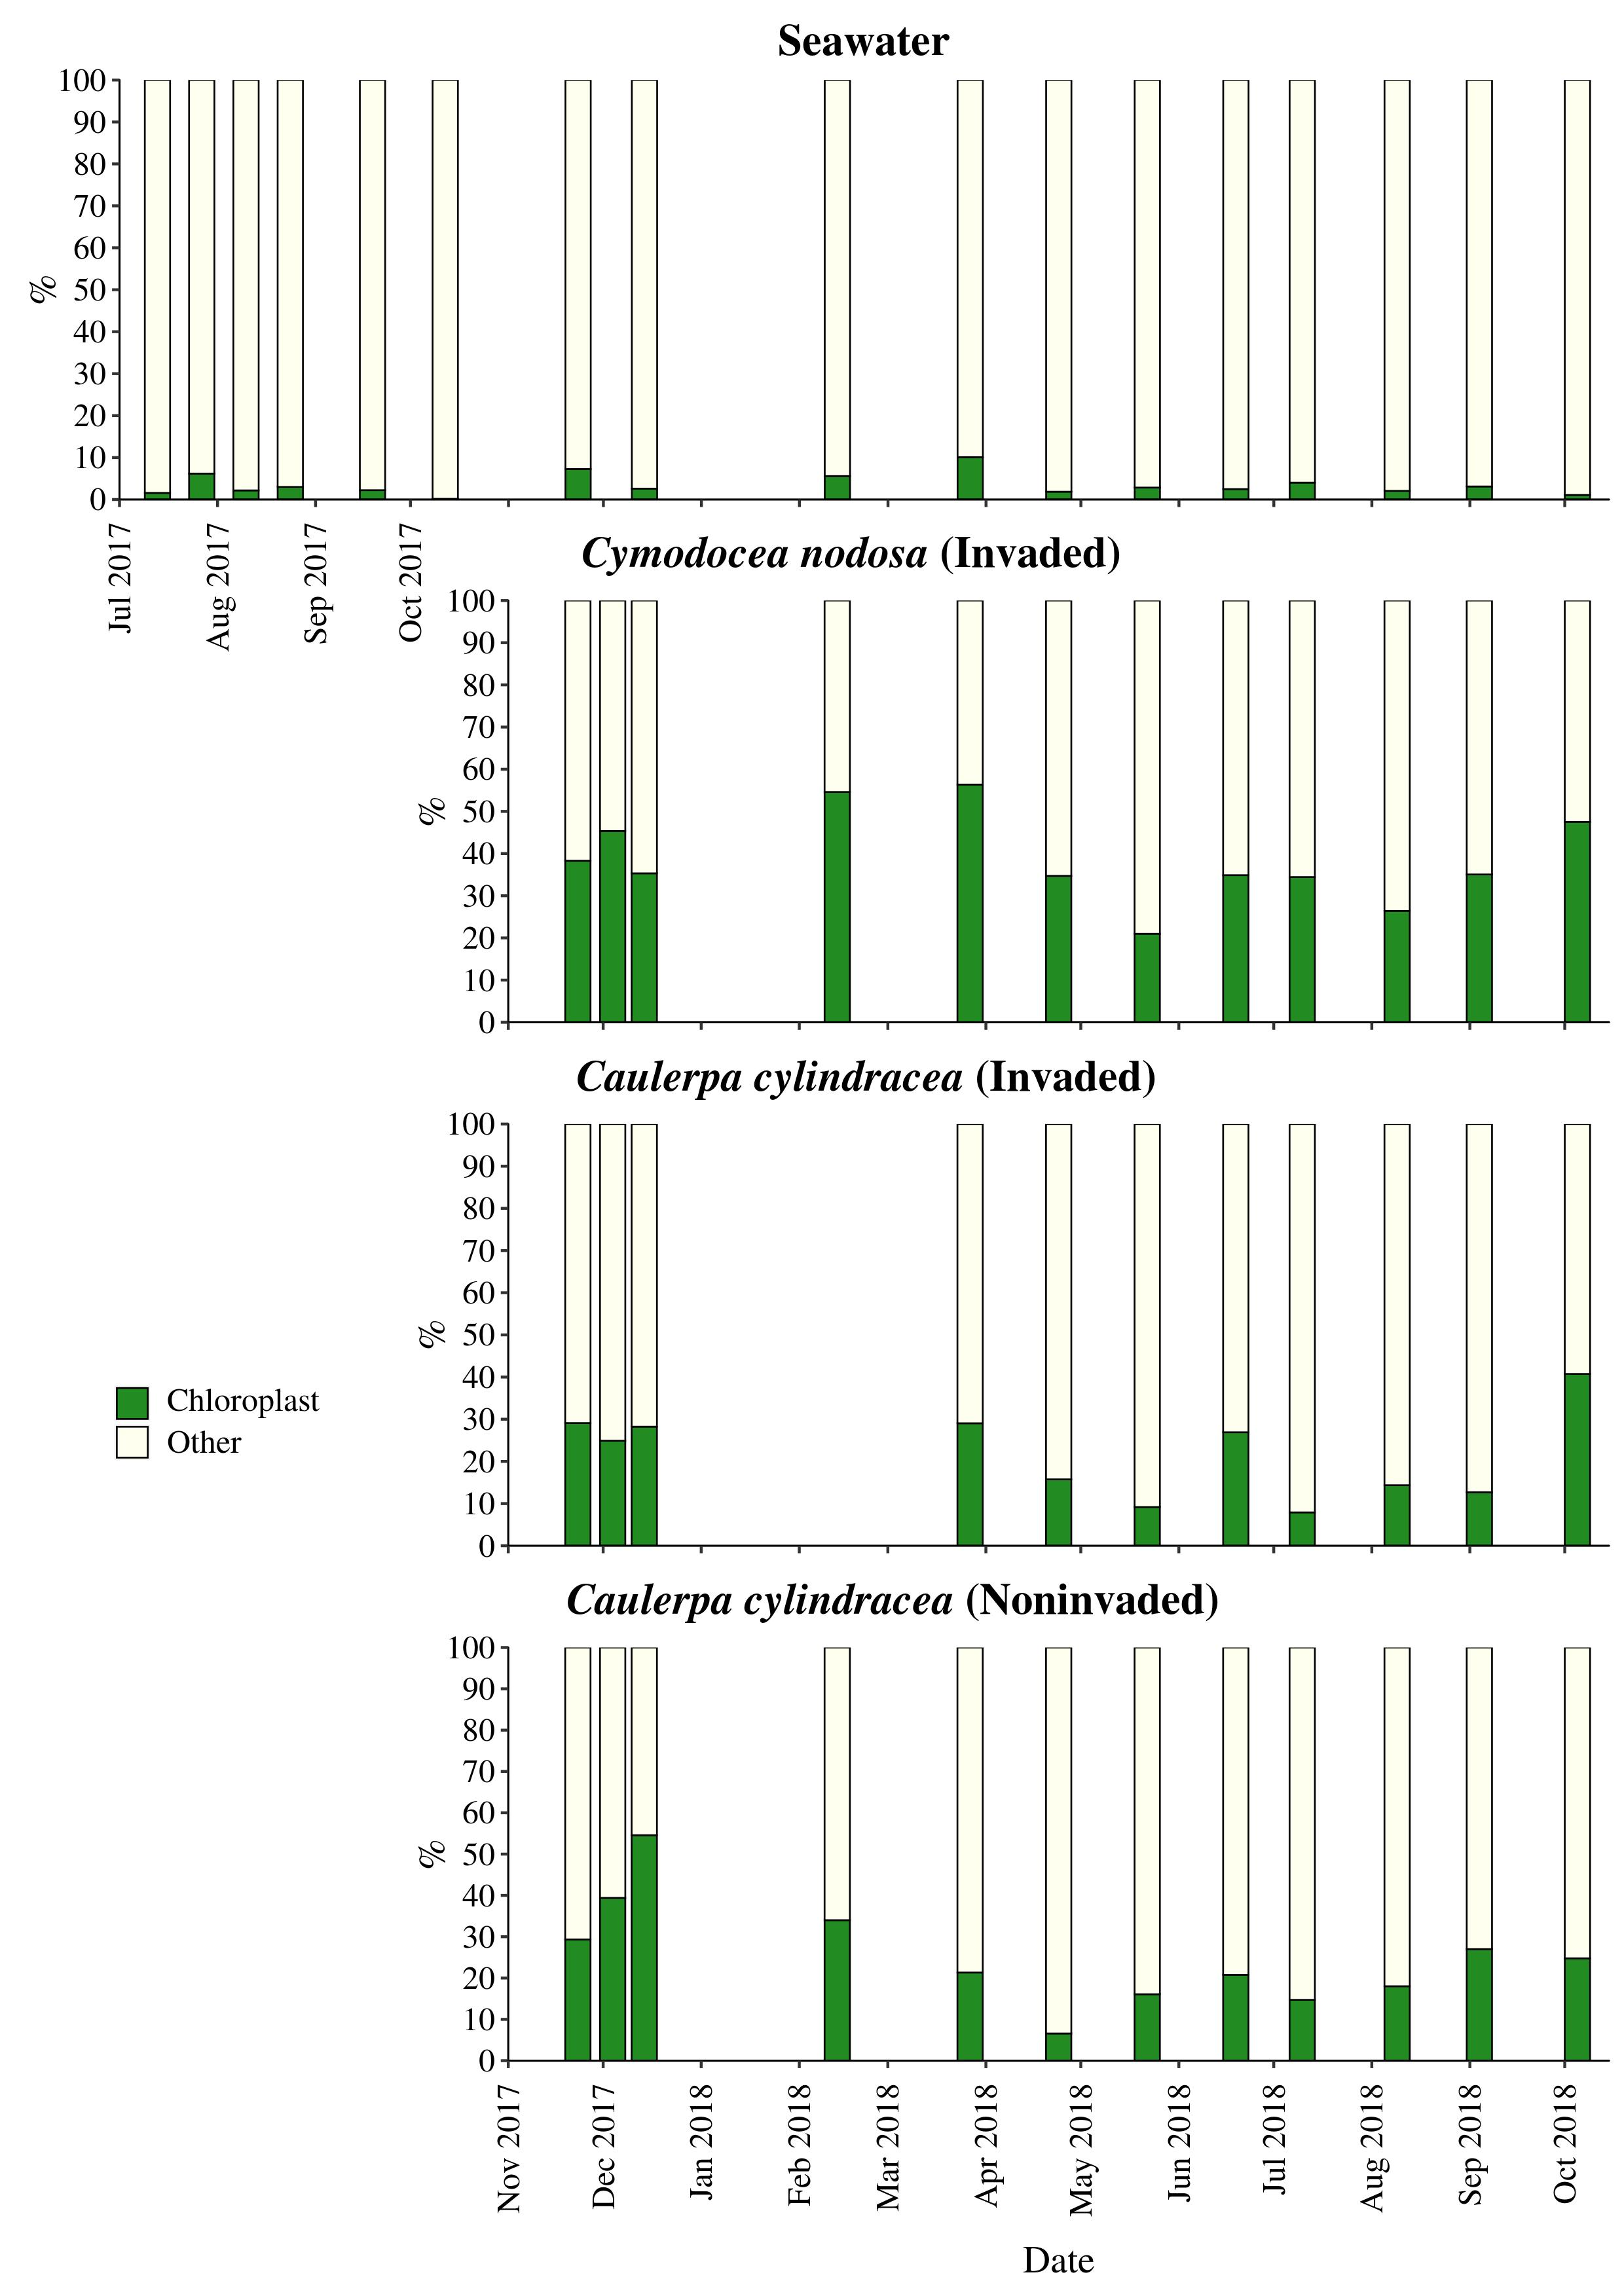
\includegraphics[width=0.85\linewidth]{../results/figures/chloroplast_bar_plot} 

}

\caption{Relative contribution of chloroplast sequences on the surfaces of macrophytes (\textit{Cymodocea nodosa} [Invaded] and \textit{Caulerpa cylindracea} [Invaded and Noninvaded]) and in the surrounding seawater.\label{chloroplast}}\label{fig:unnamed-chunk-3}
\end{figure}

\hypertarget{supplementary-table}{%
\subsection{Supplementary Table}\label{supplementary-table}}

\begingroup\fontsize{9}{11}\selectfont

\begin{longtable}{>{\centering\arraybackslash}p{6em}ccccc}
\caption{\label{tab:nseq_notus}Sample ID, Community Type, Sampling Date and Season, No. of Sequences and No. of OTUs of each sample.\label{nseq_notus}}\\
\toprule
\textbf{Sample ID} & \textbf{Community Type} & \textbf{Date} & \textbf{Season} & \textbf{No. of Sequences} & \textbf{No. of OTUs}\\
\midrule
\endfirsthead
\caption[]{Sample ID, Community Type, Sampling Date and Season, No. of Sequences and No. of OTUs of each sample.\label{nseq_notus} \textit{(continued)}}\\
\toprule
\textbf{Sample ID} & \textbf{Community Type} & \textbf{Date} & \textbf{Season} & \textbf{No. of Sequences} & \textbf{No. of OTUs}\\
\midrule
\endhead
\
\endfoot
\bottomrule
\endlastfoot
3 & Seawater & 13 July 2017 & Summer & 25,988 & 820\\
5 & Seawater & 27 July 2017 & Summer & 58,955 & 993\\
7 & Seawater & 10 August 2017 & Summer & 32,622 & 847\\
9 & Seawater & 24 August 2017 & Summer & 60,932 & 1,060\\
11 & Seawater & 19 September 2017 & Summer & 46,106 & 1,168\\
13 & Seawater & 12 October 2017 & Autumn & 30,941 & 974\\
15 & Seawater & 23 November 2017 & Autumn & 27,585 & 1,187\\
17 & Seawater & 14 December 2017 & Autumn & 44,598 & 2,267\\
19 & Seawater & 13 February 2018 & Winter & 44,185 & 1,313\\
21 & Seawater & 27 March 2018 & Winter & 46,305 & 1,565\\
23a & Seawater & 24 April 2018 & Spring & 30,962 & 1,005\\
23b & Seawater & 24 April 2018 & Spring & 38,556 & 1,201\\
25 & Seawater & 22 May 2018 & Spring & 53,876 & 1,787\\
27 & Seawater & 19 June 2018 & Spring & 77,465 & 1,288\\
29 & Seawater & 10 July 2018 & Summer & 50,799 & 1,452\\
31 & Seawater & 9 August 2018 & Summer & 39,041 & 1,119\\
33 & Seawater & 4 September 2018 & Summer & 36,195 & 1,206\\
35 & Seawater & 5 October 2018 & Autumn & 49,584 & 1,013\\
37 & \textit{Cymodocea nodosa} (Invaded) & 23 November 2017 & Autumn & 31,236 & 1,554\\
41 & \textit{Cymodocea nodosa} (Invaded) & 4 December 2017 & Autumn & 24,237 & 1,175\\
45 & \textit{Cymodocea nodosa} (Invaded) & 14 December 2017 & Autumn & 32,683 & 1,056\\
49 & \textit{Cymodocea nodosa} (Invaded) & 13 February 2018 & Winter & 9,086 & 1,215\\
52 & \textit{Cymodocea nodosa} (Invaded) & 27 March 2018 & Winter & 17,004 & 1,217\\
55 & \textit{Cymodocea nodosa} (Invaded) & 24 April 2018 & Spring & 42,645 & 2,061\\
58 & \textit{Cymodocea nodosa} (Invaded) & 22 May 2018 & Spring & 21,337 & 1,289\\
61 & \textit{Cymodocea nodosa} (Invaded) & 19 June 2018 & Spring & 31,729 & 2,099\\
64 & \textit{Cymodocea nodosa} (Invaded) & 10 July 2018 & Summer & 35,731 & 1,795\\
67 & \textit{Cymodocea nodosa} (Invaded) & 9 August 2018 & Summer & 26,364 & 2,126\\
70 & \textit{Cymodocea nodosa} (Invaded) & 4 September 2018 & Summer & 23,278 & 1,728\\
73 & \textit{Cymodocea nodosa} (Invaded) & 5 October 2018 & Autumn & 29,911 & 2,209\\
38 & \textit{Caulerpa cylindracea} (Invaded) & 23 November 2017 & Autumn & 36,316 & 2,900\\
42 & \textit{Caulerpa cylindracea} (Invaded) & 4 December 2017 & Autumn & 28,373 & 3,253\\
46 & \textit{Caulerpa cylindracea} (Invaded) & 14 December 2017 & Autumn & 34,711 & 3,059\\
53 & \textit{Caulerpa cylindracea} (Invaded) & 27 March 2018 & Winter & 28,690 & 2,488\\
56 & \textit{Caulerpa cylindracea} (Invaded) & 24 April 2018 & Spring & 34,784 & 3,067\\
59 & \textit{Caulerpa cylindracea} (Invaded) & 22 May 2018 & Spring & 23,393 & 2,720\\
62 & \textit{Caulerpa cylindracea} (Invaded) & 19 June 2018 & Spring & 36,483 & 3,322\\
65 & \textit{Caulerpa cylindracea} (Invaded) & 10 July 2018 & Summer & 18,487 & 2,196\\
68 & \textit{Caulerpa cylindracea} (Invaded) & 9 August 2018 & Summer & 31,960 & 3,112\\
71 & \textit{Caulerpa cylindracea} (Invaded) & 4 September 2018 & Summer & 29,290 & 3,170\\
74 & \textit{Caulerpa cylindracea} (Invaded) & 5 October 2018 & Autumn & 11,700 & 1,710\\
39 & \textit{Caulerpa cylindracea} (Nonnvaded) & 23 November 2017 & Autumn & 22,081 & 2,437\\
43 & \textit{Caulerpa cylindracea} (Nonnvaded) & 4 December 2017 & Autumn & 13,665 & 1,894\\
47 & \textit{Caulerpa cylindracea} (Nonnvaded) & 14 December 2017 & Autumn & 8,407 & 1,465\\
51 & \textit{Caulerpa cylindracea} (Nonnvaded) & 13 February 2018 & Winter & 11,674 & 1,909\\
54 & \textit{Caulerpa cylindracea} (Nonnvaded) & 27 March 2018 & Winter & 39,470 & 3,143\\
57 & \textit{Caulerpa cylindracea} (Nonnvaded) & 24 April 2018 & Spring & 20,300 & 2,831\\
60 & \textit{Caulerpa cylindracea} (Nonnvaded) & 22 May 2018 & Spring & 33,042 & 3,312\\
63 & \textit{Caulerpa cylindracea} (Nonnvaded) & 19 June 2018 & Spring & 41,844 & 3,978\\
66 & \textit{Caulerpa cylindracea} (Nonnvaded) & 10 July 2018 & Summer & 27,037 & 2,693\\
69 & \textit{Caulerpa cylindracea} (Nonnvaded) & 9 August 2018 & Summer & 26,738 & 3,142\\
72 & \textit{Caulerpa cylindracea} (Nonnvaded) & 4 September 2018 & Summer & 31,868 & 3,267\\
75 & \textit{Caulerpa cylindracea} (Nonnvaded) & 5 October 2018 & Autumn & 33,066 & 3,099\\*
\end{longtable}
\endgroup{}


\end{document}
